\intermediate{\subsection{Downloading the programs}}

\step{Downloading the programs.}{
    Download \program{BEAST} from \href{http://beast2.org}{\url{http://beast2.org}} and install it on your computer.
    This tutorial is written for the Mac OS X version of \program{BEAST}v2.6.5.
    
    You will be using \program{BEAST} to run \program{SNAPPER}, although it is possible to run \program{SNAPPER} on its own. However, you 
    have to use \program{BEAST} in order to combine \program{SNAPPER} and marginal likelihood estimation into the same analytical framework. 
    Thus, without \program{BEAST} you would not be able to conduct species delimitation with \program{SNAPPER}.
    }

\step{Data included with the tutorial.}{
   After downloading and unzipping this archive you should have a SNAPPER-delimitation-tutorial folder on your computer. This tutorial contains the files and folders shown in
    Box~\ref{box:tutorialDir}. The \menutab{data} folder contains the gecko SNP data in binary format (necessary for \program{SNAPPER}). If you are unsure of how to convert your own
    SNP data from nucleotide to binary format, please read the documentation \href{http://beast2.org/tutorials/}{A rough guide to SNAPP} (Section 4. Preparing Input File). You can find scripts for converting SNP data into \program{SNAPPER} input format at our phrynomics project site at \href{https://github.com/bbanbury/phrynomics}{GitHub}. You can also find help
    at the \program{BEAST} \href{https://groups.google.com/forum/?fromgroups\#!forum/beast-users}{google users group}.
    The \menutab{xml} folder contains seven xml files (named according to the species delimitation models in Figure~\ref{fig:map}) that are ready to run in \program{BEAST}. 

    \begin{textbox}
        \centering
        \fbox{\begin{minipage}[c][15em][c]{0.5\textwidth}
            \ttfamily
            \begin{compactitem}
                \item SNAPPER-delimitation-tutorial/
            \begin{compactitem}
                	\item SNAPPER-delimitation-tutorial.pdf
                    \item data/
                       \begin{compactitem}
                        \item hemi129.nex
                        \item smallhemi129.nex
                    \end{compactitem}
                    \item xml/
                    \begin{compactitem}
                        \item runA.xml
                        \item runB.xml
                        \item runC.xml
                        \item runD.xml
                        \item runE.xml
                        \item runF.xml
                        \item runG.xml
                    \end{compactitem}
            \end{compactitem}
            \end{compactitem}
        \end{minipage}}
        \caption{The files included in this tutorial. The data folder contains the SNP data in binary format. Ready-to-run XML files are included in the xml folder.}
        \label{box:tutorialDir}
    \end{textbox}
}

\intermediate{\subsection{Setting up the XML file with \program{BEAUTi}}}

\step{Launch BEAUTi}{Begin by launching the \program{BEAUTi} program that comes with \program{BEAST}. If you
    are using Mac OSX or Windows, you should be able to do this by double
    clicking on the application. If everything is working correctly, a window
    should appear that looks something like Figure~\ref{fig:beautiInit}.
    \begin{figure}[htbp]
        \centering
        \fbox{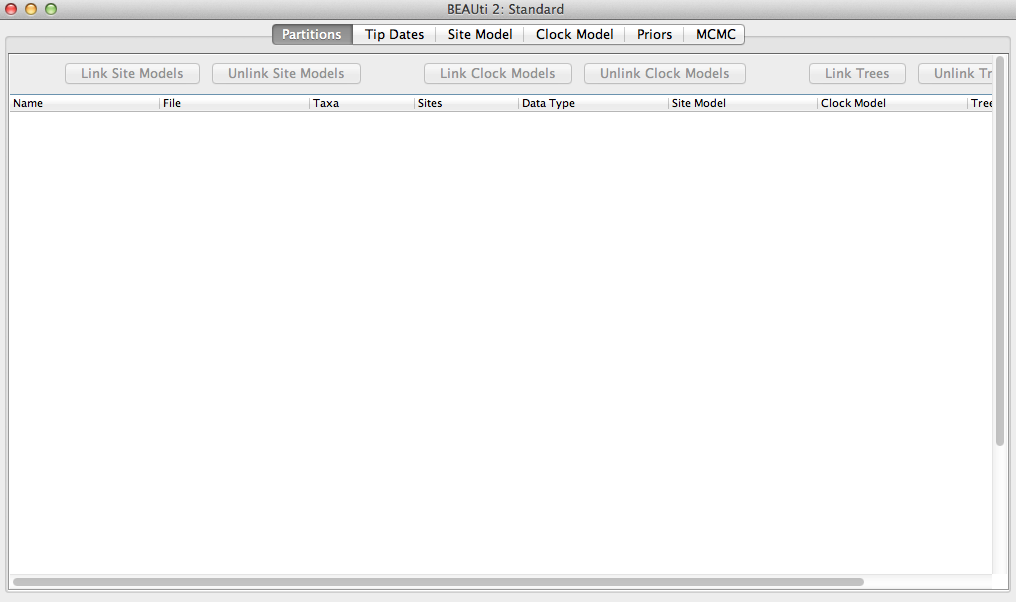
\includegraphics[width=0.7\textwidth]{../../BFD*/screenshots/beauti-init.png}}
        \caption{BEAUTi window launched from \program{BEAST}.}
        \label{fig:beautiInit}
    \end{figure}
}

\step{Install SNAPPER and model selection packages}{You need to add functionality to \program{BEAST} in order to estimate 
     species trees with SNP data and 
     to perform model selection. Begin by using the drop-down 
     menu \subItem{File}{Manage Packages.} A window should 
     appear that looks something like Figure~\ref{fig:beauti-manage-packages}.
     Select and install the packages \program{{\bf SNAPPER}} and \program{{\bf Model\_Selection}}. You can then exit the 
     window by clicking the {\bf ``Close''} button.
    \begin{figure}[htbp]
        \centering
        \fbox{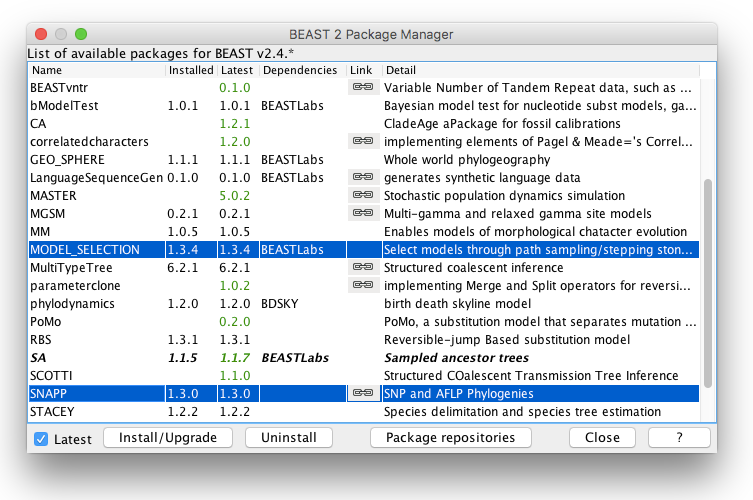
\includegraphics[width=0.7\textwidth]{../../BFD*/screenshots/beauti-manage-packages.png}}
        \caption{\program{BEAUTi} package manager for \program{BEAST}.}
        \label{fig:beauti-manage-packages}
    \end{figure}

}

\step{Converting \program{BEAUTi} to \program{SNAPPER} mode}{Tell \program{BEAUTi} that you are  
     setting up a \program{SNAPPER} analysis, which will change the menu options and allow us to import SNP data.
     Begin by using the drop-down 
     menu \subItem{File}{Template, SNAPPER.} 
     This should change the appearance of the \program{BEAUTi} 
     window to look something like Figure~\ref{fig:beauti-SNAPPER}.

    \begin{figure}[htbp]
        \centering
        \fbox{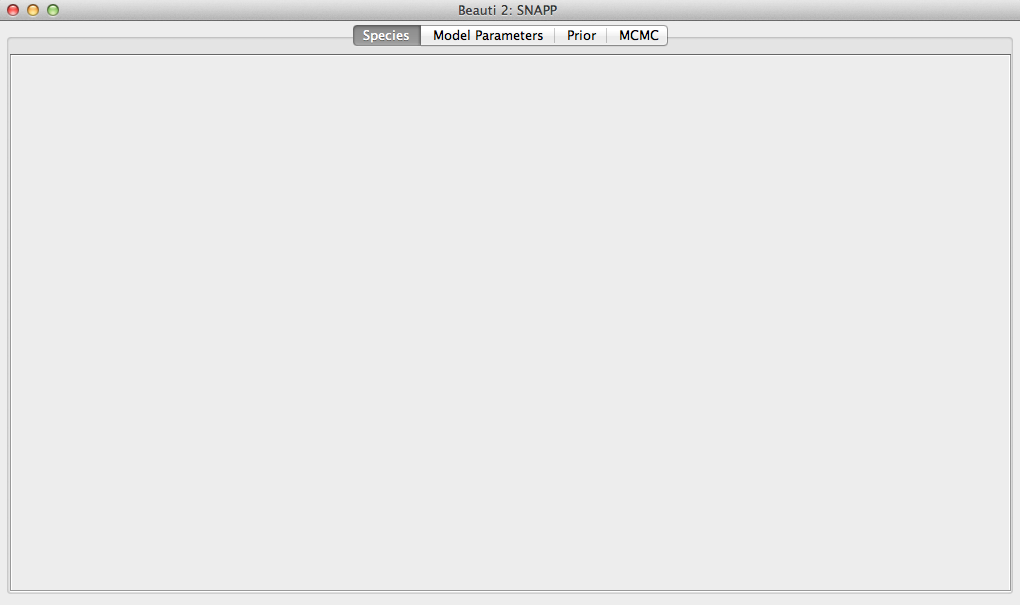
\includegraphics[width=0.7\textwidth]{../../BFD*/screenshots/beauti-snapp.png}}
        \caption{\program{BEAUTi} window after importing the \program{SNAPPER} template. Notice that the menu tabs have changed.}
        \label{fig:beauti-SNAPPER}
    \end{figure}

}


\step{Import the SNP data.}{
    Import the SNP data (the {\bf smallhemi129.nex} file)
    using the drop-down menu \subItem{File}{Import Alignment.}
    
    {\em NB if you load the full data set from {\bf hemi129.nex} instead you might not finish this tutorial in the allocated time frame.}

    Once the data are successfully loaded into \program{BEAUTi} you should see a list of the 
    samples included in the data file (Figure~\ref{fig:beauti-data-imported}.)

    \begin{figure}[htbp]
        \centering
        \fbox{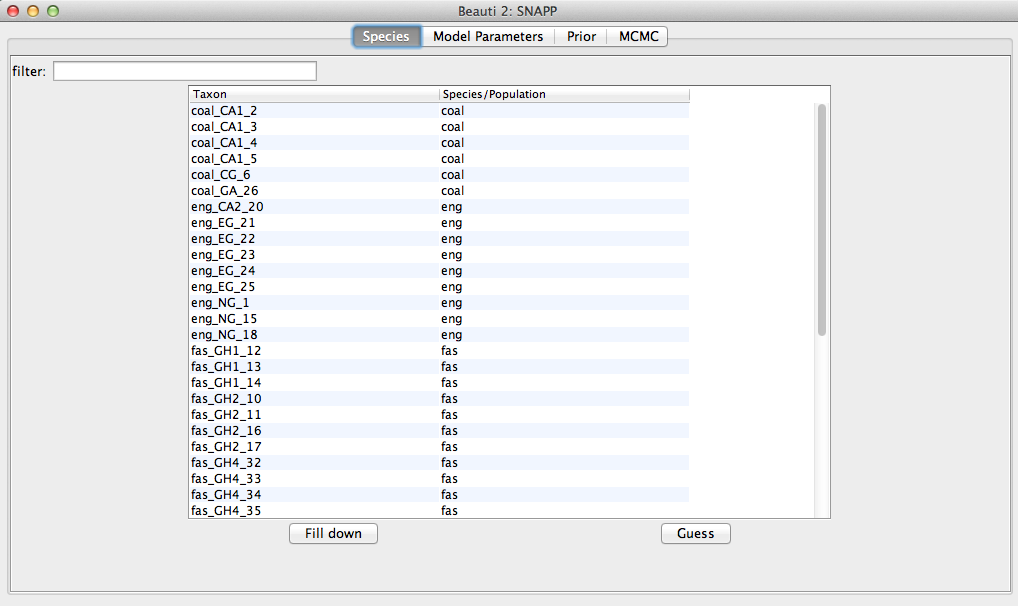
\includegraphics[width=0.8\textwidth]{../../BFD*/screenshots/beauti-data-imported.png}}
        \caption{The data successfully loaded by BEAUTi.}
        \label{fig:beauti-data-imported}
    \end{figure}
}

\step{Define species.}{
    There are several ways to designate species assignments. You can automatically 
    designate species names using the names already 
    present in the data files. The species names can be pre-defined this way by including a ``delimiter'' that 
    allows the species name to be parsed from the rest of the sequence name. The gecko data 
    file uses an underscore ``\_'' to separate
    the species name (on the left) from the rest of the sequence name (on the right) as follows:\\
    \\
    \cmd{eng\_NG\_1}\\ 	
    \cmd{coal\_CA1\_2}\\	
    \cmd{coal\_CA1\_3}\\
    \cmd{coal\_CA1\_4}\\	
    \cmd{coal\_CA1\_5}\\	
    \cmd{coal\_CG\_6}\\	
    \cmd{kya\_GH3\_7}\\	
    \cmd{kya\_GH3\_8}\\	
    \cmd{\ldots}\\
    \\
    Other options for assigning species names are available using the ``Guess'' button. The screen should look similar to 
     Figure~\ref{fig:beauti-guess-trait}. 
     
    How many samples should you include? The number of samples slows down SNAPPER much more than the number of SNPs. Therefore, if your analyses are going too slow, then it is typically better to randomly subsample down to an even proportion of sequences from each species instead of removing SNPs. Reducing the number of samples by half will more than half the analysis time. When setting up a new analysis, start with a small number of samples for each species (for example, 4 samples per species), which will enable you to make quicker progress. Increase the number of samples once your analyses are returning reasonable results. If you are overambitious with your sampling, then your analyses will become unbearably slow. 

    \begin{figure}[htbp]
        \centering
        \fbox{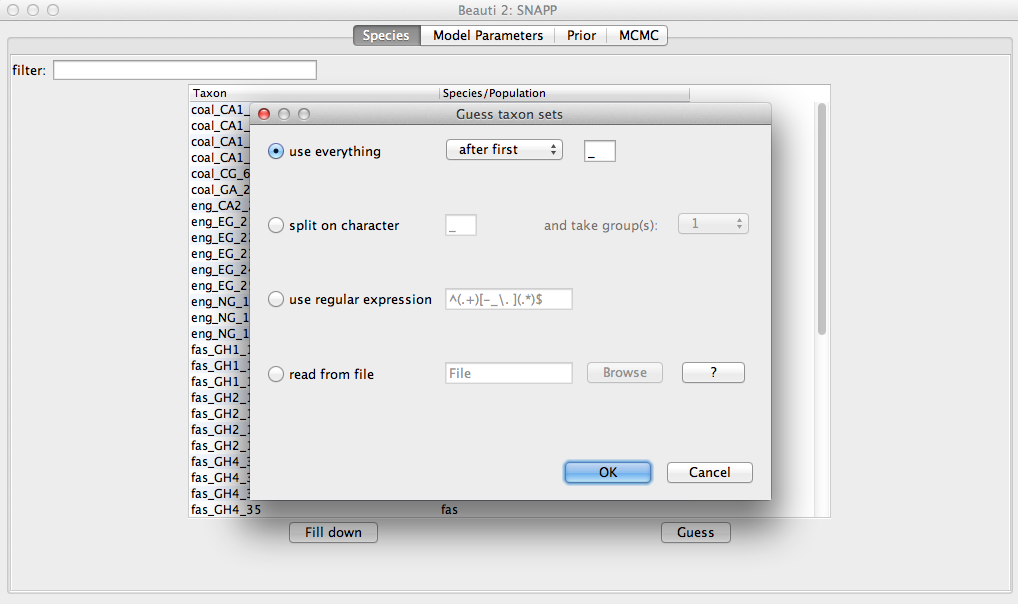
\includegraphics[width=0.8\textwidth]{../../BFD*/screenshots/beauti-guess-trait.png}}
        \caption{The species assignment options that appears after you select the ``Guess' button.}
        \label{fig:beauti-guess-trait}
    \end{figure}
 
    You can import a custom mapping file that links each sample to a species using the ``read from file'' option.      
    Click the ``Ok'' button to return to the \menutab{Species} window. Be sure that each Taxon has a Species/Population name.    
}


\step{Set the mutation model.}{
    Next, set up our model under the \menutab{Mutation Model} tab Figure~\ref{fig:beauti-mutation}.
    Be sure to read the documentation \href{http://www.beast2.org/tutorials}{A rough guide to SNAPPER} to learn more about the model options. Briefly, the parameters are as follows:

\small{
    \begin{compactdesc}
       \item[\field{Mutation Rate U: instantaneous rate of mutating from the 0 allele to the 1 allele.}]
       \item[\field{Mutation Rate V: instantaneous rate of mutating from the 1 allele to the 0 allele.}]
       \item[\field{Coalescence Rate: population size parameter with one value for each node in the tree.}]
    \end{compactdesc}
    
    \textit{Recommendations:}  Set mutation rates u and v = 1 and do not sample. Alternatively, you can click the {\bf ``Calc mutation rates''} button to get a direct estimate of u and v. Either way, you typically do not have to estimate these parameters during the MCMC. 
    Coalescent Rate: check the sample box. If you do not sample, then you assume that all population sizes are the same, which is unrealistic. The coalescent rate is 2/theta, and the number is simply the starting value used to initialize the analysis. Do not confuse the coalescent rate with the theta prior. The theta prior is described in detail in the next section.
    
    The ``Include non-polymorphic'' checkbox is used in cases where invariant sites have been included in the data. The likelihood calculations are 
    different if \program{SNAPPER} assumes that all constant sites have been removed. If you are using a typical SNP dataset that only includes variable site, then make sure that the box is not checked.
    
    The ``Mutation Only At Root'' checkbox indicates conditioning on zero mutations, except at root (default false). As a result, all gene 
    trees will coalesce in the root only, and never in any of the branches. This option is allows you to emulate the model used by \citet{nielsen1998} and \citet{roychoudhury2008}.
    
    The ``Show Pattern Likelihoods And Quit'' checkbox is handy if you just want to print out the likelihoods for all patterns in the starting state and then quit.
    
    The ``Use Log Likelihood Correction'' checkbox is for calculating corrected likelihood values for Bayes factor test of different species assignments (the calculation is almost instantaneous, and it will not slow down your analysis).
        
    }
    
        \begin{figure}[htbp]
        \centering
        \fbox{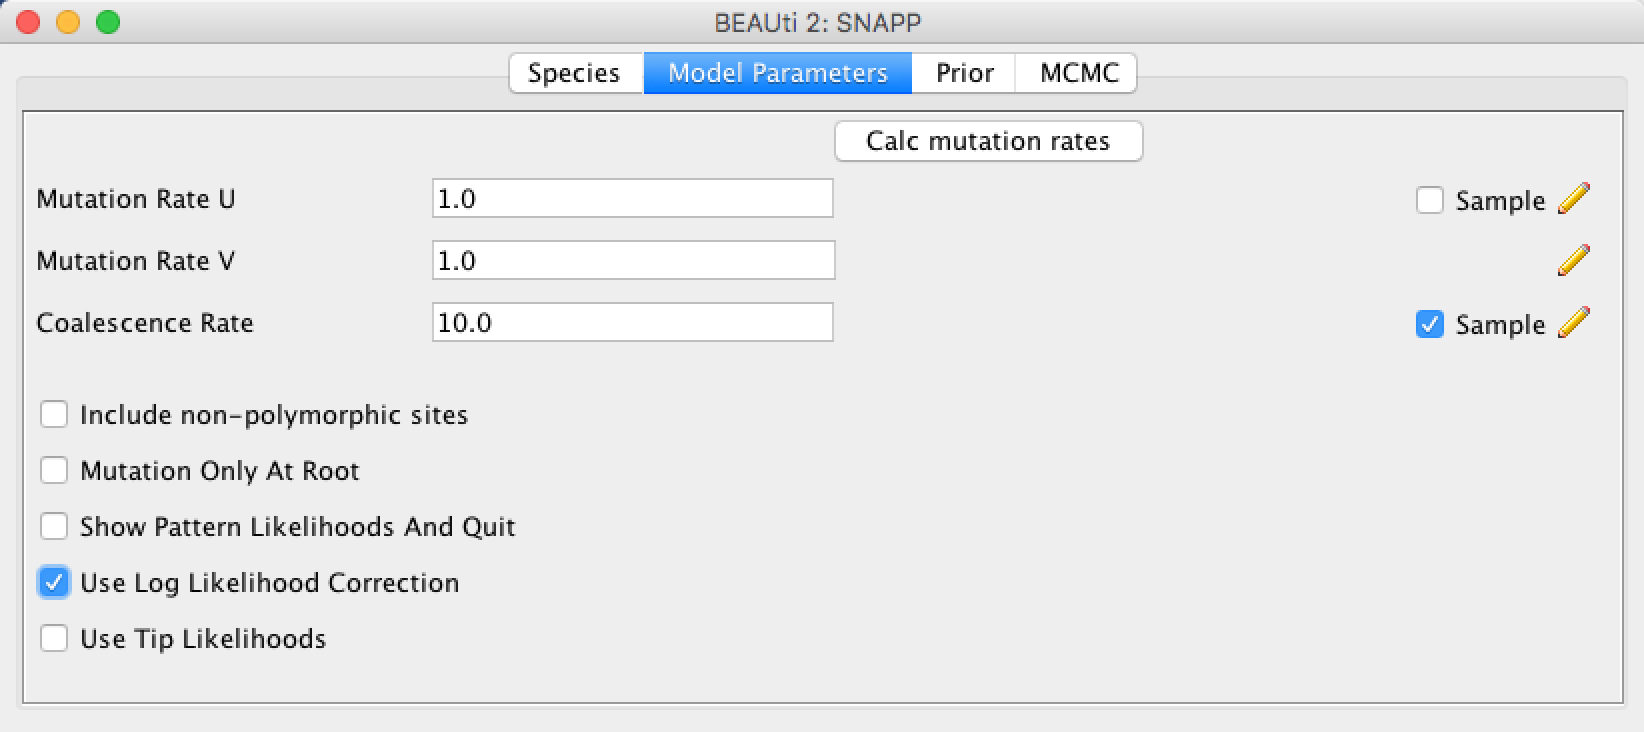
\includegraphics[width=0.8\textwidth]{../../BFD*/screenshots/beauti-mutation.png}}
        \caption{The Mutation Model options.}
        \label{fig:beauti-mutation}
    \end{figure}
}

    
\step{Define the priors.}{
    Next, move to the \menutab{Prior} tab and specify the priors (Figure~\ref{fig:beauti-prior}.) Again, read the 
    documentation \href{http://www.beast2.org/tutorials}{A rough guide to SNAPPER} 
    to learn more about these priors. It is important to be aware of the biological meaning of these priors. 
    One problem with \program{SNAPPER} is that it is deceptively easy to set up an analysis using default options. 
    However, setting it up right requires thinking about details that some empiricists would rather not think about.

\small{
    \begin{compactdesc}
       \item[\field{Alpha: shape parameter for the gamma prior on population sizes.}]
       \item[\field{Beta: rate parameter for the gamma prior on population sizes.}]
       \item[\field{Kappa: parameter used when selecting the CIR rate prior (below).}]
       \item[\field{Lambda: Birth rate for the Yule model prior on the species tree.}]
       \item[\field{Rateprior: prior on rates can be Gamma, InverseGamma, CIR, or Uniform.}]
    \end{compactdesc}
}

\textit{Setting the expected divergence (theta) prior.} Recall that for a diploid population, theta = 4Nu, where N is the effective population size and u is the per-generation mutation rate. If theta=0.004, you expect to observe 0.4\% variation between two randomly sampled alleles in a population. Another way to think about this is in the expected number of substitutions; ``theta=0.004'' means that for two randomly sampled individuals within a population you expect to observe 4 SNPs in 1,000 bases. In \program{BEAUTi}, the gamma prior on theta is parameterized such that the mean is alpha/beta. For example, if alpha=1 and beta = 250, the prior mean on theta is 0.004. One way of estimating a reasonable mean for the theta prior is to calculate pairwise sequence divergence among all individuals known to belong to a single species and take the average value as the mean for theta. Higher prior means on theta will favor models with populations grouped together, because they represent an expectation that average divergence within populations is relatively high. Users can select different distributions for the theta prior under ``Rateprior''. If ``Rateprior'' is set to ``gamma'' (recommended), the mean value of theta is calculated as alpha/beta.  Note that in some implementations (including the R function rgamma() and Beauti's internal visualizer), the mean of a gamma distribution is calculated as alpha*beta rather than alpha/beta. This is the case for the Lambda prior (discussed below). Finally, kappa is a parameter that is only applied when the CIR distribution is used (see the Rough Guide to SNAPPER for further details). 

\textit{Setting the speciation rate prior Lambda:} \program{SNAPPER} uses a Yule prior for the species tree and branch lengths on the species tree. This prior has a single parameter, {$\lambda$} (Lambda), representing the speciation rate. This rate, in turn, determines the (prior) expected height of the species tree. The higher the speciation rate, the higher the probability of supporting more species during species delimitation. The trees that come out of SNAPPER are not time calibrated. The branch lengths should be interpreted in units of expected substitutions per site. Translating this into time requires an assumption about the substitution rate. Two different options for setting lambda are compared in this tutorial: using a fixed value versus assigning a broad prior. In general, tree height estimates are similar using either a fixed lambda (lambda = 5) or a gamma distribution (2, 200), as shown below. The mean of the gamma distribution for Lambda is calculated as alpha*beta rather than alpha/beta as it is for theta. 

     \begin{figure}[htbp]
        \centering
        \fbox{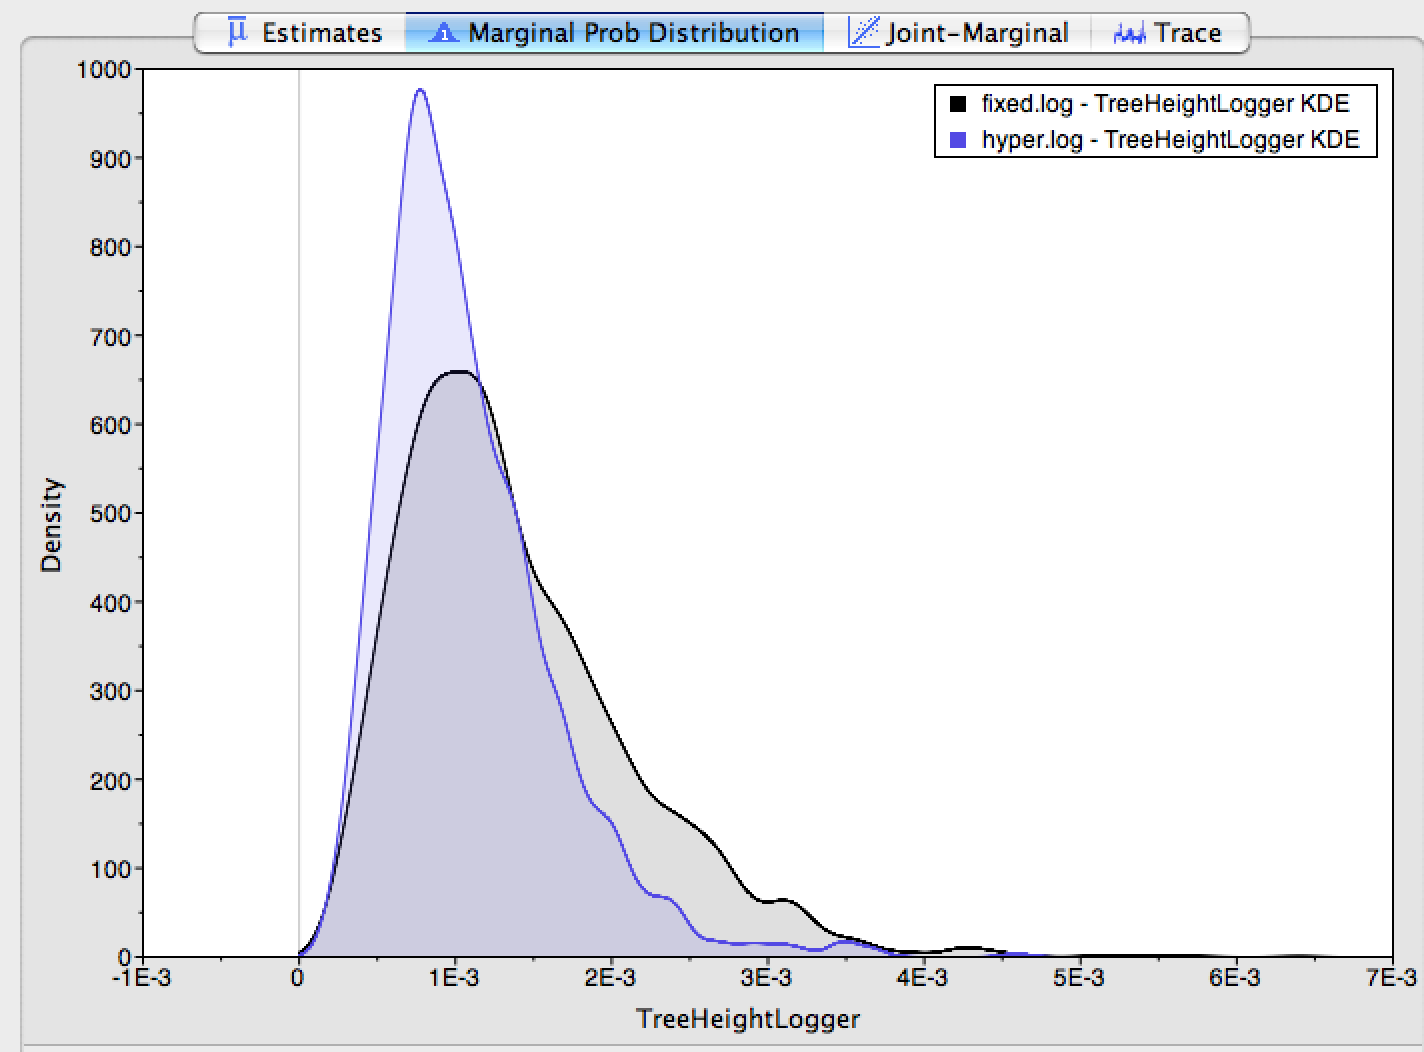
\includegraphics[width=0.8\textwidth]{../../BFD*/screenshots/lambda_comparision.png}}
        \caption{Tree height comparison of analyses using a fixed lambda (lambda = 5) versus a hyperprior on lambda (gamma {$\sim$} 2,200). The plot shows the marginal probability distributions superimposed for the two estimates, which overlap broadly suggesting that the estimates are quite similar.}
        \label{fig:lambda_comparision}
    \end{figure}  
    
    
\textit{Fixed value for Lambda}: The specific prior that you use for {$\lambda$} (Lambda) depends on the number of species in your analysis and the depth of your tree in units of expected substitutions per site. See the Rough Guide to SNAPPER for further details and an equation for calculating Lambda. Using a useful script written by Jamie Oaks, called \href{https://github.com/joaks1/pyule}{pyule}, you can calculate an appropriate lambda value based on prior information about the number of species, and the height of the species tree in expected substitutions per site. If sequence data are available, then you can approximate the height of the species tree obtained by calculating the maximum observed divergence between any pair of taxa divided by two (height = max divergence/2). 
   \newpage
Table 1 provides some suggestions for Lambda priors across a range of expected substitutions per site from root to tip (up to 20\% sequence divergence from root to any tip), and for relatively small species trees (up to 20 species). In general, different Lambda settings do not influence the results, since in most cases the data will dominate. 

Table 1: Lambda prior settings across a range of species tree heights (in expected substitutions per site) and sizes (number of species).
\begin{table}[ht]
\tabcolsep=0.4cm
\begin{tabular}{rrcccccc}
\hline
        &    & \multicolumn{6}{c}{Species tree height (expected substitutions per site)}     \\
        				&    	& 0.001 	& 0.005 	& 0.01 	& 0.05  	& 0.10 	&0.2\\
        				&    	&  (0.1\%)	&  (0.5\%) &  (1\%) 	&  (5\%)  	& (10\%)  	& (20\%)\\ \hline
        				& 2 	& 500	& 100 	& 50 		& 10 		& 5 		& 0.2\\
Number of species 	& 5	& 1283 	& 257 	& 128 	& 26 		& 13 		& 6\\
        				& 10	& 1928 	& 386 	& 193 	& 39 		& 19 		& 10\\
        				& 15	&  2318	&  464	&  232	& 46		& 23		& 12\\
        				& 20	&  2598	&  520	&  260	& 52 		& 26 		& 13\\\hline
\end{tabular}
\end{table}
    
    \begin{figure}[htbp]
        \centering
        \fbox{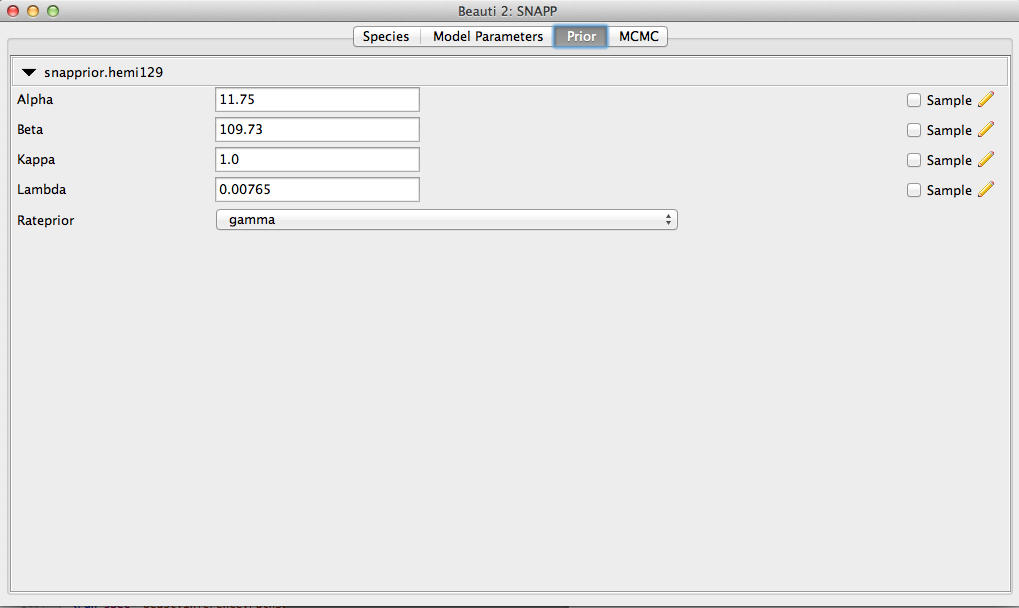
\includegraphics[width=0.8\textwidth]{../../BFD*/screenshots/beauti-prior.png}}
        \caption{The prior settings option 1: using a fixed value for Lambda.}
        \label{fig:beauti-prior}
    \end{figure}   

\textit{Gamma distribution for Lambda}: You also have the option of using a hyperprior for lambda to accommodate uncertainty in the parameter (sampling lambda is the default setting). However, the default setting is an improper prior (1/X), which is useless for species delimitation. The 1/X prior is not a proper probability distribution, and you cannot rely on the path-sampling results. Instead, use a gamma prior with a broad distribution, for example, alpha = 2 and beta = 200. The mean of the gamma distribution for Lambda is calculated as alpha*beta rather than alpha/beta as it is for theta. If there is prior information about the number of expected substitutions, then this could be used to set up the prior. Try setting the mean of the gamma distribution to be somewhere in the middle of the extreme lambda values (shown in Table 1) that apply to your study system. 

    \begin{figure}[htbp]
        \centering
        \fbox{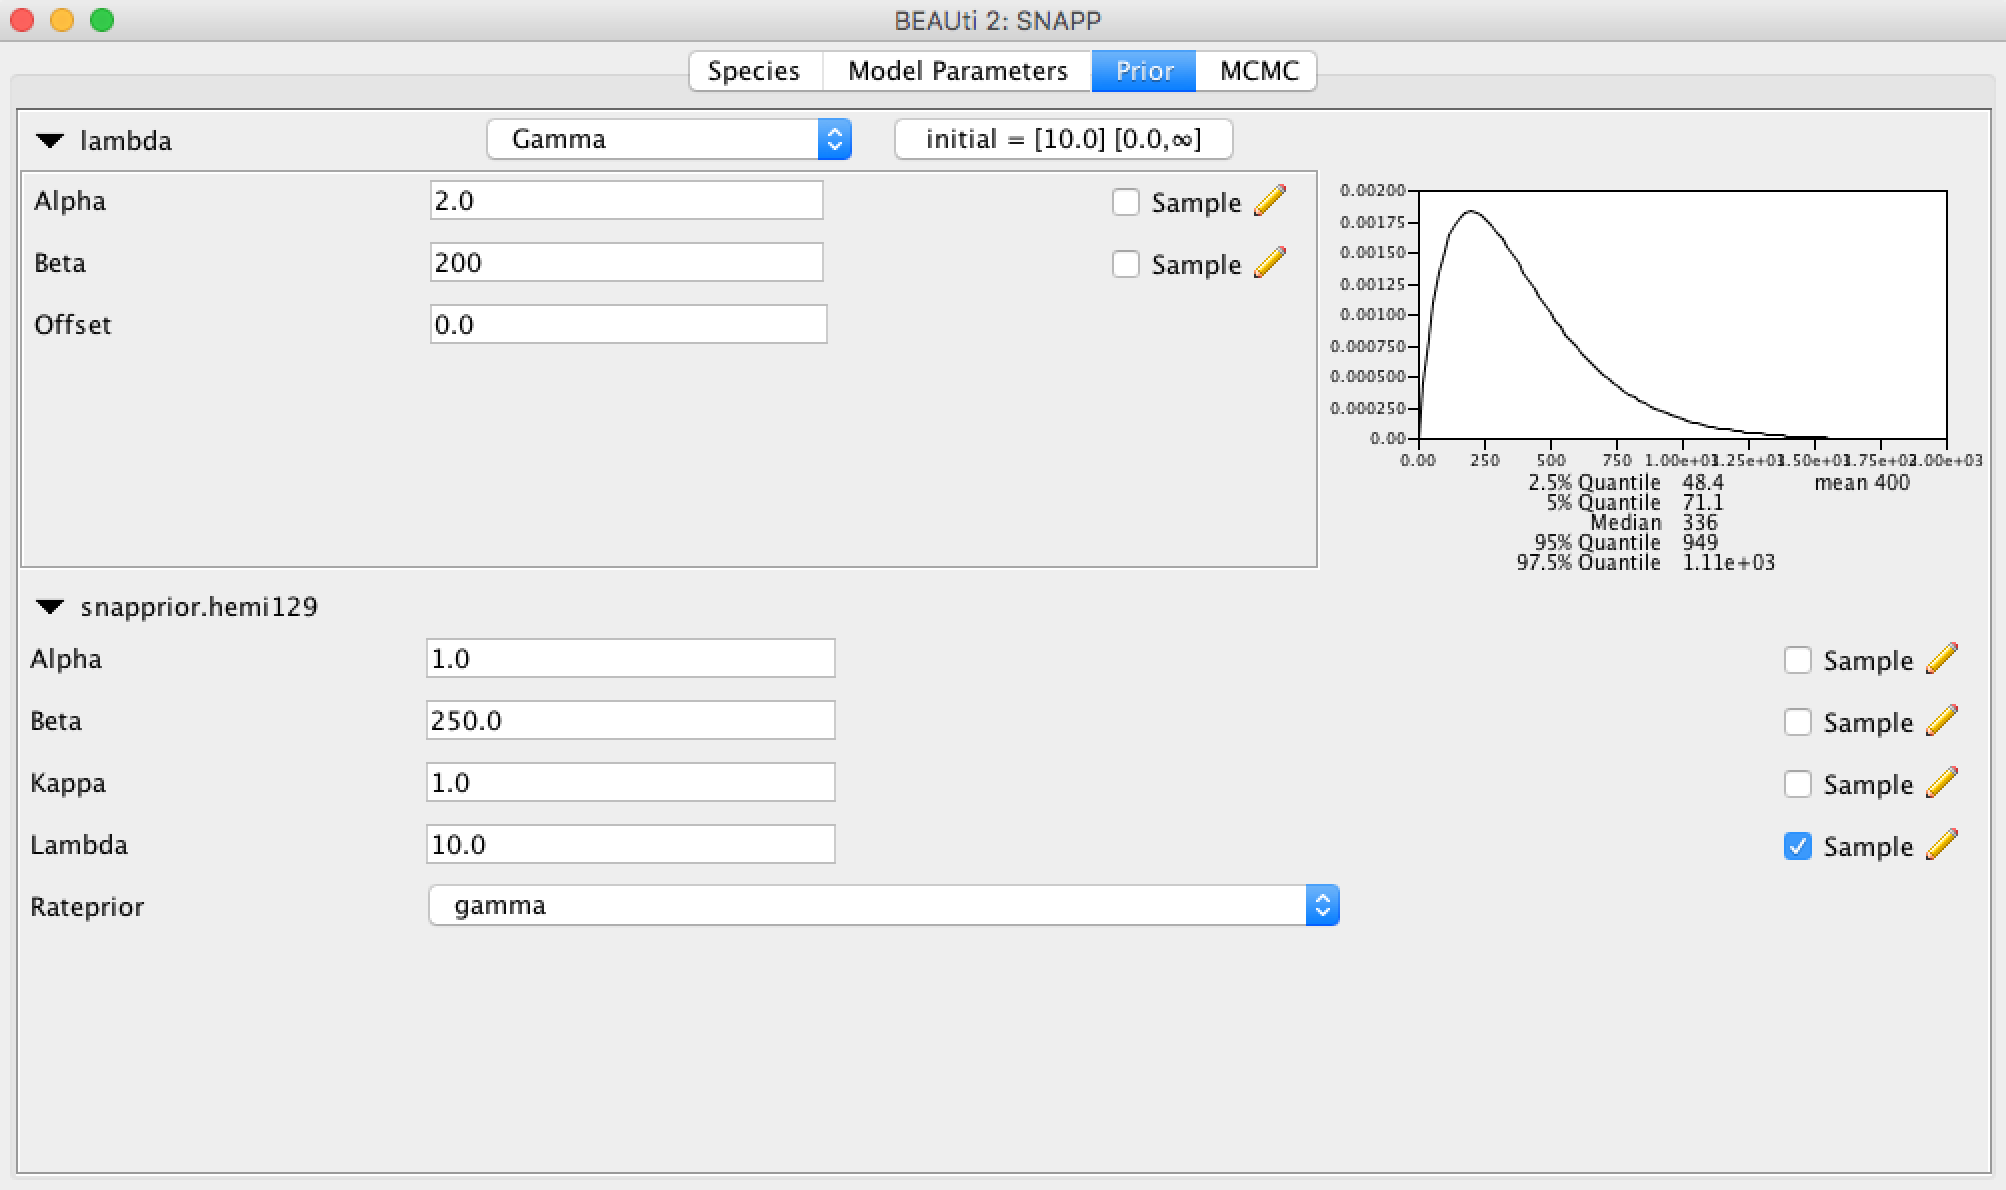
\includegraphics[width=0.8\textwidth]{../../BFD*/screenshots/beauti-prior2.png}}
        \caption{The prior settings option 2: using a gamma prior for Lambda.}
        \label{fig:beauti-prior2}
    \end{figure}   
    
    }

   
%   \newpage
   


\step{Specify MCMC settings and generate the XML file.}{
    Next, move to the \menutab{MCMC} tab. 
    Change the following settings:
    \begin{compactdesc}
        \centering
        \item[\field{State Burnin:}] \fieldvalue{0}
        \item[\field{Chain Length:}] \fieldvalue{1000}
        \item[\field{Store Every:}] \fieldvalue{10}
        \item[\field{tracelog:File Name:}] \fieldvalue{runA.log}
        \item[\field{tracelog:Log Every:}] \fieldvalue{10}
        \item[\field{treelog:File Name:}] \fieldvalue{runA.trees}
        \item[\field{treelog:Log Every:}] \fieldvalue{10}
    \end{compactdesc}
    Leave the remaining options at their default values
    (Figure~\ref{fig:beauti-mcmc}). These MCMC values are way to low, and a thorough analysis requires much more computational time. 
    The MCMC run times are intentionally kept short (and the data files reduced) in this tutorial. These short analyses should run in approximately 2 -- 4 minutes depending
    on the number of processors available on your computer.  
    Thorough analyses of the full data takes 2 -- 6 days, depending on the number of species in the model, and generally require at least 100,000 generations. Running multiple independent analyses  using different starting seeds and comparing results is a good way to ensure that the analyses are converging.
 
    \begin{figure}[htbp]
        \centering
        \fbox{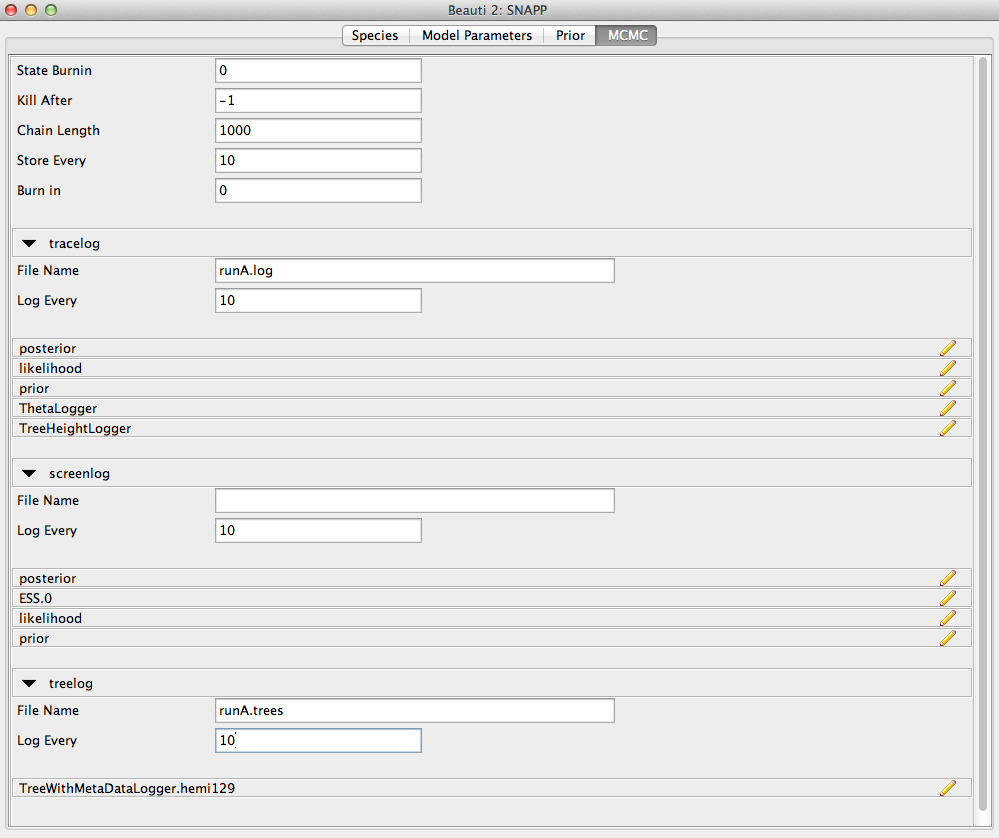
\includegraphics[width=1.0\textwidth]{../../BFD*/screenshots/beauti-mcmc.png}}
        \caption{The MCMC settings.}
        \label{fig:beauti-mcmc}
    \end{figure}

    Next, save the file using \subItem{File}{Save\ldots.} 
    Another subwindow will appear for specifying the name and location for
    saving the XML file. Name the file ``runA.xml'' and place it in a folder with the same name.
    Save the file to
    the \localfile{SNAPPER-delimitation-tutorial} folder.\\
    }

\intermediate{\subsection{Running the stepping stone analysis with \program{BEAST}}}

\step{Setting up for marginal likelihood estimation.}{
There are two ways to set up the stepping stone analysis; through a GUI, and by editing the XML. The GUI is more convenient but makes it a bit harder to transfer the analysis to a cluster, and since stepping stone analyses are typically very computational intensive, it often makes sense to run them on a cluster. In this step, we explain how to set up the analysis using the GUI, and in the next two steps it is explained how to set up an XML file through a text editor.

First, start the BEAST app-store by selecting the File/Launch apps menu in BEAUti (alternatively, double click the AppStore icon in the BEAST folder). A window similar to Figure~\ref{fig:appstore} should pop up.

    \begin{figure}[htbp]
        \centering
        {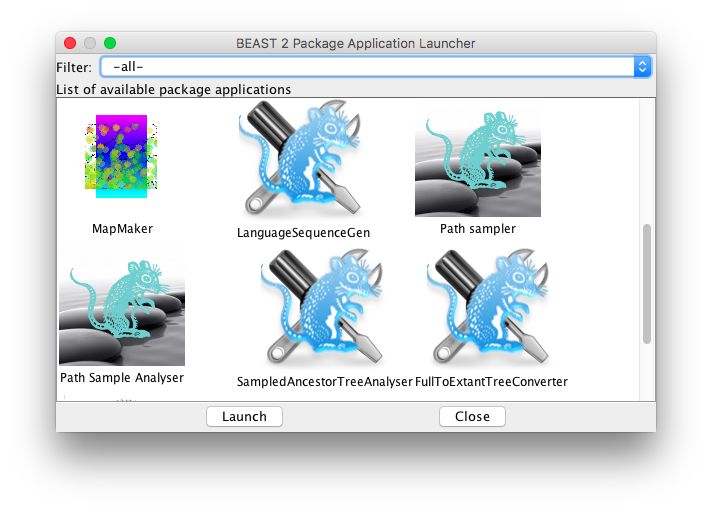
\includegraphics[width=0.6\textwidth]{../../BFD*/screenshots/appstore}}
        \caption{BEAST app store.}
        \label{fig:appstore}
    \end{figure}

Select the Path sampler icon, and hit the Launch button. A new window pops up with the GUI for path sampling/stepping stone analysis similar to Figure~\ref{fig:pathsampler}. 

If you prefer to start from the command line, you can use the following in a terminal:

    	    \cmd{/path/to/BEASTv2.4.5/bin/appstore PathSampler}

Select the file with MCMC analysis you just set up in BEAUti, and change the settings as indicated in Figure~\ref{fig:pathsampler}.

    \begin{figure}[htbp]
        \centering
        {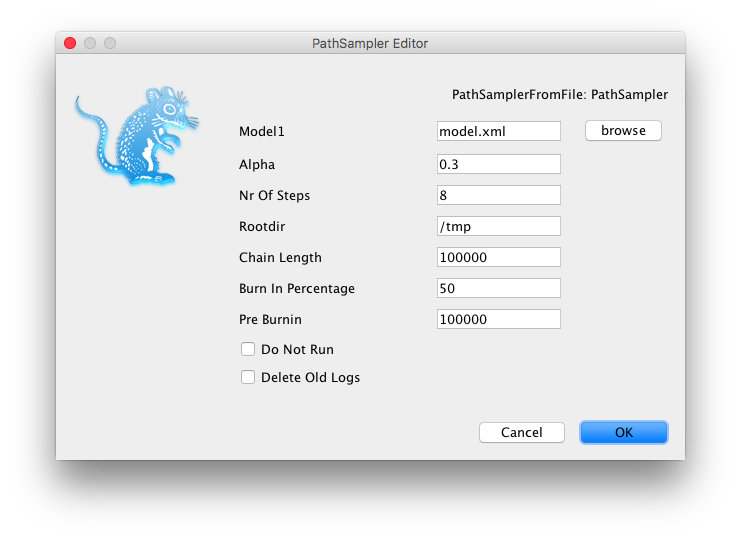
\includegraphics[width=0.7\textwidth]{../../BFD*/screenshots/pathsampler}}
        \caption{GUI for path sampling/stepping stone analysis.}
        \label{fig:pathsampler}
    \end{figure}


%\intermediate{\subsection{Editing the XML file for marginal likelihood estimation}}

{\bf Step 11b}{Editing the XML file for marginal likelihood estimation.}
Species delimitation using SNPs requires marginal likelihood estimation. 
You will need to edit the XML file to prepare it for analysis in \program{BEAST}. Instructions for setting up
marginal likelihood estimation using path sampling are provided at the \href{http://www.beast2.org/tutorials}{BEAST} website. The procedure involves (1) typing in some short codes in a few places, (2) replacing some words, and (3) copying and pasting some sections around. Specific instructions are below:
 
Open your XML file in a text editor. Search and replace the opening run statement (located about half way through the file) with an mcmc statement by changing {\bf ``<run ...>''} into {\bf ``<mcmc ...>''.} Next, type a new closing mcmc statement, {\bf ``</mcmc>''}, just before the closing run statement, {\bf ``</run>''}, located at the end of the file.

Now you are ready to insert the path sampling commands. You will need to insert the following block of text into your XML file immediately above the opening ``<mcmc ...>''' element:

\small{
\cmd{<run spec=`beast.inference.PathSampler'}\\ 
\cmd{chainLength="1000"}\\
\cmd{alpha=`0.3'}\\
\cmd{rootdir=`/home/desktop/SNAPPER-delimitation-tutorial/runA/'}\\
\cmd{burnInPercentage=`0'}\\
\cmd{preBurnin="0"}\\
\cmd{deleteOldLogs=`true'}\\ 
\cmd{nrOfSteps=`24'>}\\
\cmd{cd \$(dir)}\\
\cmd{java -cp \$(java.class.path) beast.app.beastapp.BeastMain \$(resume/overwrite) -java -seed \$(seed) beast.xml}\\
}


{\bf Important:} If you copy and paste this section into your XML file, be sure to check that the symbols paste correctly. The quote symbols (`` ` ' ") don't copy as they should, and these will cause problems. Also, make sure that the root directory path (rootdir) exists on your computer.

	These path sampling parameters are way to low, and a thorough analysis requires much more computational time. Stable marginal likelihood estimates usually require at least 48 steps (sometimes 100), chainLength = 100,000 (sometimes 1,000,000), and preBurnin=10,000 (sometimes 100,000). The MCMC run times are 
    intentionally kept short in this tutorial to obtain quick (but meaningless) results. The run time on a MacBook Pro 2.3GHz i7 processor with 16GB of memory is approximately 2.5 minutes, and this is running 8 concurrent steps (= 8 threads). Increasing the number of threads will speed up the analysis by running more concurrent path sampling steps, but this requires more memory (this analysis uses about 12GB of memory). For large-scale analyses, many users find that they run out of memory before processors.

The path sampling parameters that you just entered into your XML file are as follows:

    \begin{compactdesc}
       \item[\field{chainLength: MCMC sample length for each path sampling step.}]
       \item[\field{alpha: parameter used to space out path sampling steps.}]
       \item[\field{rootdir: directory for storing output. Be sure that the folder exists before starting the run.}]
       \item[\field{burnInPercentage: burn-In percentage used for analyzing the log files.}]
       \item[\field{preBurnin: number of samples that are discarded for the first step, but not the others.}]
       \item[\field{deleteOldLogs: delete existing log files from rootdir}]
      \item[\field{nrOfSteps: the number of path sampling steps to use}]
    \end{compactdesc}
    
If for some reason you are using an older versions of \program{SNAPPER} (<v1.1.10) you may need an extra step; find the text {\bf ``snap.MCMC''} and replace it with {\bf ``beast.core.MCMC''.}  
Finally, move the entire {\bf ``stateDistribution''} element to just before the run element. This step requires that you move all of the lines starting with {\bf ``<stateDistribution''} and ending with {\bf ``</stateDistribution>''} to just above the run element.


}

        
\intermediate{\subsection{Running the XML file with \program{BEAST}}}

\step{Run the XML file in \program{BEAST.}}{
	    You can execute the XML file in \program{BEAST} using the GUI or the command line. If you are using Mac OSX or Windows, you should 
	    be able to launch the \program{BEAST} GUI by double clicking on the application icon. 
	    After the \program{BEAST} window appears, click the \field{Choose File\ldots} button, 
	    and select the XML file you just created (Figure~\ref{fig:beast}). Increase the \field{Thread pool size} to speed up your analysis. 
	    Running SNAPPER with multiple threads can increase speeds, but experimenting with the number of threads is required to get the best performance.

	    Click \field{Run}. The analysis should take about 10 minutes. 
	    You can also run \program{BEAST} from the command line. Open the {\bf Terminal} Application and navigate to the folder 
	    containing your {\bf runA.xml} file. To execute the file, type the following at the command line:
	    
	    \cmd{/path/to/BEASTv2.4.1/bin/beast -threads 8 runA.xml}
	    
	    or
	    
	    \cmd{beast -threads 8 runA.xml}
	    
	    if you have already moved the \program{BEAST} executable to your path. Caution: setting the number of \field{threads} beyond the maximum number available on your computer can have serious drawbacks, and you will probably not have enough memory to support all of those separate analyses.
	  	
	\begin{figure}[htbp]
        \centering
        \fbox{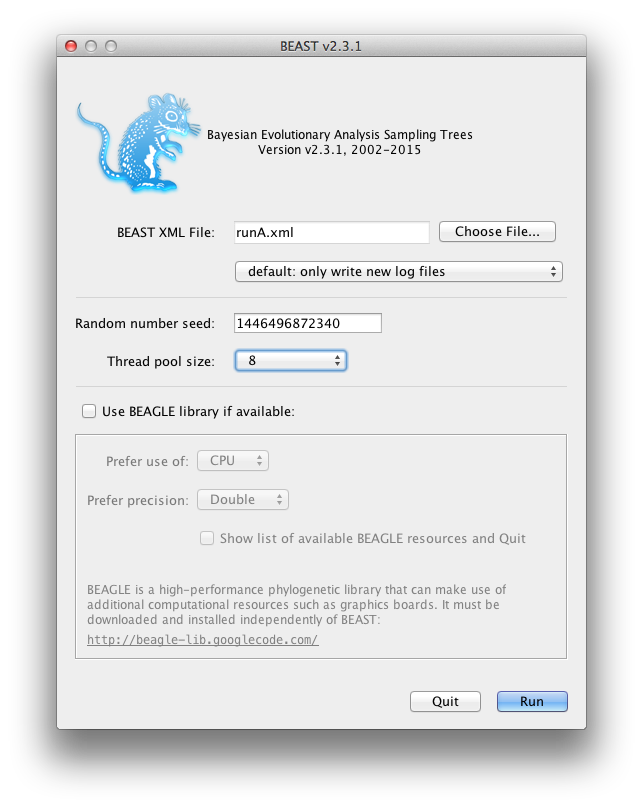
\includegraphics[width=0.5\textwidth]{../../BFD*/screenshots/beast.png}}
        \caption{The \program{BEAST} GUI window.}
        \label{fig:beast}
    \end{figure}
    }

\intermediate{\subsection{Inspecting path sampling results}}

\step{Inspecting path sampling results.}{
At the end of your analysis, the path sampling results will be displayed on the screen. An example is shown in Figure~\ref{fig:beast-output}. 
Each row shows the results from one path sampling step. The example in Figure~\ref{fig:beast-output} shows the results from a path sampling analysis with 24 steps. You will use the value after "marginal L estimate" to compare models. 

       \begin{figure}[htbp]
        \centering
        \fbox{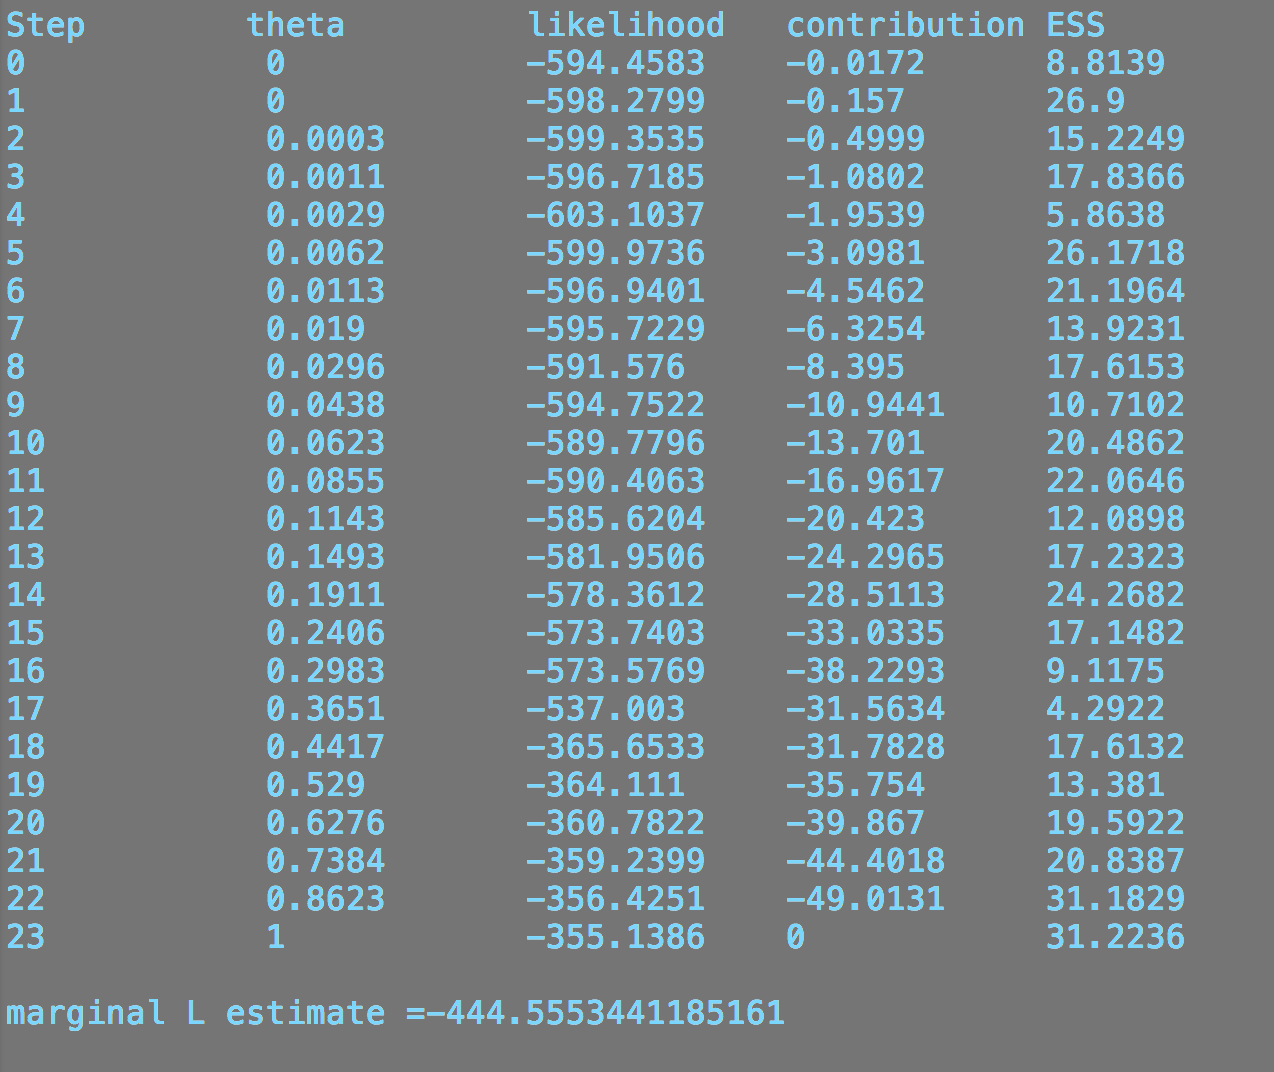
\includegraphics[width=0.5\textwidth]{../../BFD*/screenshots/beast-output.png}}
        \caption{The path sampling output at the end of the analysis.}
        \label{fig:beast-output}
    \end{figure}
}



\intermediate{\subsection{Setting up new species delimitation models}}

\step{Setting up new XML files for species delimitation.}{
Now that you have one XML file up and running it is easy to make new XML files for each species delimitation model.
To prepare a new file for species delimitation, make a few slight modifications to the existing runA.xml file: (1) save a copy of the xml file as runB.xml and save it in a new folder with the same name, (2) change the file stem names in the xml file so that you don't accidentally overwrite any of your previous results, (3) edit the path sampling root directory to point to the new runB folder, 4) change the species assignments listed in the  {\bf ``stateDistribution''} element. This last part requires changing the number and/or composition of taxonset features. Each taxonset begins with {\bf ``<taxonset ...>''} and ends with {\bf ``</taxonset>''} (Figure~\ref{fig:beast-taxon-set}). To lump species, simply combine the taxon names into a single taxonset feature. To split a species, simple create a new taxonset containing the appropriate taxon names. To reassign a taxon to another species you can cut and paste the taxon to a different taxonset. 
XML files containing the species assignments shown in Figure \ref{fig:map} are provided with this tutorial (see Box~\ref{box:tutorialDir}). The XML files included with this tutorial contain a reduced number of samples in the taxonset blocks to help speed up the analyses. You do not have to exclude the samples from the data matrix and rerun \program{BEAUTi}. It is much more efficient to simply edit the taxonset features to include only those samples that you intend to anlayze.

       \begin{figure}[htbp]
        \centering
        \fbox{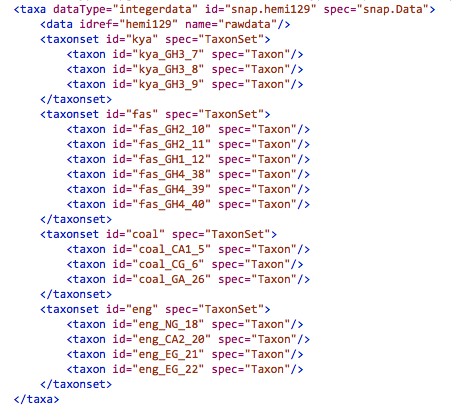
\includegraphics[width=0.5\textwidth]{../../BFD*/screenshots/beast-taxon-set.png}}
        \caption{Example of the taxonset features in the XML file.}
        \label{fig:beast-taxon-set}
    \end{figure}
}


\step{Comparing species delimitation models with Bayes factors.}{  
   After you run each of the alternative species delimitation models you can rank them by their marginal likelihood estimate (MLE). You 
   can also calculate Bayes factors to compare the models. 
   The Bayes factor (BF) is a model selection tool that is simple and well suited for the purposes of comparing species delimitation models. 
   Calculating the BF between models is simple. To do so, simply subtract the MLE values for two models, and then multiply the difference by two (BF = 2 x (model1 - model2). A positive BF value indicates support in favor of model 1. A negative BF value indicates support in favor of model 2. 

The strength of support from BF comparisons of competing models can be evaluated using the framework of \cite{kass95}. 
 The BF scale is as follows: 
0 < BF < 2 is not worth more than a bare mention, 2 < BF < 6 is positive evidence, 6 < BF < 10 is strong support, and BF > 10 is decisive.

The results for the seven gecko models are provided in Table 2. The model that lumps the western forests into one species (runB) is the top-ranked model. It has the largest MLE value, and it is supported in favor of the current taxonomy model (runA). The BF in support for model B is decisive compared to model A. It is important to emphasize that these results are \textit{tragically deficient} in terms of the MCMC analysis. Much, much longer runs are required to obtain stable results. 

Table 2: Path sampling results for the seven species delimitation models shown in Figure \ref{fig:map}. All Bayes factor (BF) calculations are made against the current taxonomy model (runA). Therefore, positive BF values indicate support for the current taxonomy model, and negative BF values indicate support for the alternative model.
\begin{table}[ht]
\tabcolsep=0.2cm
\begin{tabular}{l c c c c } 
\hline     
Model 							& Species 	& MLE 	& Rank 		& BF\\\hline
runA, current taxonomy				& 4 			& -935.820	& 5		& --\\
runB, lump western forests			& 3 			& -898.914	& 1		& -73.8\\
runC, lump central forests				& 3 			& -963.806	& 7		& +56.0\\
runD, lump western \& central forests	& 2 			& -935.930	& 6		& +0.2\\
runE, split \textit{fasciatus}			& 5 			& -924.466	& 4		& -22.7\\
runF, split \textit{eniangii} 				& 5 			& -919.750	& 2		& -32.1\\
runG, reassign Bioko Island			& 4 			& -920.018	& 3 		& -31.6\\\hline
\end{tabular}\\
MLE = Marginal likelihood estimate\\
BF = Bayes factor\\
\end{table}
}

\intermediate{\subsection{Summarizing the trees using \program{TreeAnnotator}.}}

\step{Summarize the species tree using \program{TreeAnnotator}.}{
TreeAnnotator will summarize the posterior distribution of species trees and identify the topology with the best posterior support, and summarize the divergence times for each node in the tree.
	Launch the \program{TreeAnnotator} program.
    You can also specify the burnin value if you haven't already excluded burn-in samples in \program{LogCombiner}.
	For the \field{Target tree type} field, choose \fieldvalue{Maximum clade credibility tree}.
    For the \field{Node heights} field, choose \fieldvalue{Median heights}.
	Select the \field{Input Tree File} button and select the file \localfile{runA.trees}. When conducting path sampling, SNAPPER generates a posterior distribution of trees for each path sampling step. You will typically only want to summarize the tree file in the folder corresponding to theta=1, since the other folders contain trees that were estimated with modified likelihoods. Check the SNAPPER screen output to verify which path sampling step corresponds to theta=1 (this changes with different versions of SNAPPER).
	Select the \field{Output File} button and specify the \localfile{output} directory and a file name, \localfile{runA-MCC.tre}.
	Click \field{Run}
}

\intermediate{\subsection{Visualizing the tree in \program{FigTree}}}

\step{Visualize the species tree in \program{FigTree}.}{
    Launch the \program{FigTree} program, and load the \localfile{runA-MCC.tre} file
    you just created with \program{TreeAnnotator}.
    Check the \field{Branch Labels} option and select
    \fieldvalue{posterior} for the \subItem{Branch labels}{Display} fields.
    Check the \field{Node Bars} option and select
    \fieldvalue{height\_95\%\_HPD} for the \subItem{Node bars}{Display} field.
 
 
 You can also get a summary of some tree statistics using the TreeSetAnalyser, which you can launch from the BEAST app launcher, and looks something like Figure~\ref{fig:treesetanalyser}
       \begin{figure}[htbp]
        \centering
        \fbox{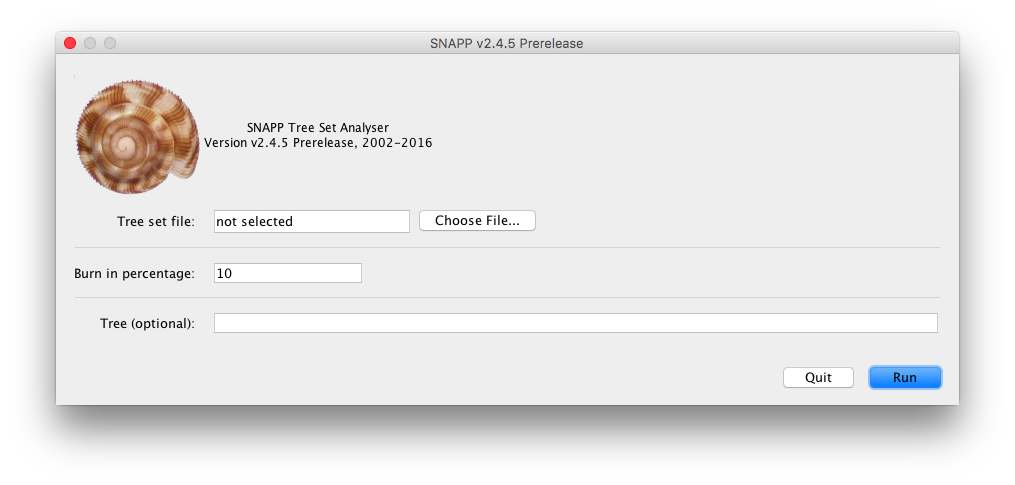
\includegraphics[width=0.5\textwidth]{../../BFD*/screenshots/treesetanalyser.png}}
        \caption{Tree set analyser utility.}
        \label{fig:treesetanalyser}
    \end{figure}
     }




